\documentclass[aspectratio=169]{beamer}
\usetheme{Bruno}
\usepackage{amsmath}
\usepackage{amssymb}
\usepackage{siunitx}
\usepackage{float}
\usepackage{tikz}
\def\checkmark{\tikz\fill[scale=0.4](0,.35) -- (.25,0) -- (1,.7) -- (.25,.15) -- cycle;} 
\usepackage{url}
\usepackage[siunitx,american,RPvoltages]{circuitikz}
\ctikzset{capacitors/scale=0.7}
\ctikzset{diodes/scale=0.7}
\usepackage{tabularx}
\newcolumntype{C}{>{\centering\arraybackslash}X}
\renewcommand\tabularxcolumn[1]{m{#1}}% for vertical centering text in X column
\usepackage{tabu}
\usepackage[spanish,es-tabla,activeacute]{babel}
\usepackage{babelbib}
\usepackage{booktabs}
\usepackage{pgfplots}
\usepackage{hyperref}
\hypersetup{colorlinks = true,
            linkcolor = black,
            urlcolor  = blue,
            citecolor = blue,
            anchorcolor = blue}
\usepgfplotslibrary{units, fillbetween} 
\pgfplotsset{compat=1.16}
\usepackage{bm}
\usetikzlibrary{arrows, arrows.meta, shapes, 3d, perspective, positioning,mindmap,trees,backgrounds}
\renewcommand{\sin}{\sen} %change from sin to sen
\usepackage{bohr}
\setbohr{distribution-method = quantum,insert-missing = true}
\usepackage{elements}
\usepackage{verbatim}
\usepackage[edges]{forest}
\usepackage{etoolbox}
\usepackage{schemata}
\usepackage{appendix}
\usepackage{listings}

\definecolor{color_mate}{RGB}{255,255,128}
\definecolor{color_plas}{RGB}{255,128,255}
\definecolor{color_text}{RGB}{128,255,255}
\definecolor{color_petr}{RGB}{255,192,192}
\definecolor{color_made}{RGB}{192,255,192}
\definecolor{color_meta}{RGB}{192,192,255}
\newcommand\diagram[2]{\schema{\schemabox{#1}}{\schemabox{#2}}}

\definecolor{codegreen}{rgb}{0,0.6,0}
\definecolor{codegray}{rgb}{0.5,0.5,0.5}
\definecolor{codepurple}{rgb}{0.58,0,0.82}
\definecolor{backcolour}{rgb}{0.95,0.95,0.92}

\lstdefinestyle{mystyle}{
    backgroundcolor=\color{backcolour},   
    commentstyle=\color{codegreen},
    keywordstyle=\color{magenta},
    numberstyle=\tiny\color{codegray},
    stringstyle=\color{codepurple},
    basicstyle=\ttfamily\footnotesize,
    breakatwhitespace=false,         
    breaklines=true,                 
    captionpos=b,                    
    keepspaces=true,                 
    numbers=left,                    
    numbersep=5pt,                  
    showspaces=false,                
    showstringspaces=false,
    showtabs=false,                  
    tabsize=2
}

\lstset{style=mystyle}
\title{Electricidad I: \\ \emph{Leyes básicas}}
\author{
    Juan J. Rojas
}
\institute{Instituto Tecnológico de Costa Rica}
\date{\today}
\background{fig/background.jpg}
\begin{document}
\sisetup{unit-math-rm=\mathrm,math-rm=\mathrm} % change sinitx font
\sisetup{output-decimal-marker = {,}}
\maketitle

\begin{frame}{Corriente, Voltaje y Resistencia}
    \begin{center}
        \begin{tabularx}{12cm}{C C C}
        \toprule
        Variable & Derivación & Unidades \\
        \midrule
        Corriente & $i = \frac{dq}{dt}$ & \si{\ampere} [\si{\coulomb \second^{-1}}] \\[5pt]
        Voltaje & $v = \frac{dw}{dq}$ & \si{\volt} [\si{\joule \coulomb^{-1}}] \\[5pt]
        Potencia & $p = v \cdot i =  \frac{dw}{dt}$ & \si{\watt} [\si{\joule \second^{-1}}] \\[5pt]
        Energía & $w = \int_{t_0}^{t_f}p\,dt$ & \si{\watt\hour} [\SI{3600}{\joule}] \\[5pt]
        \bottomrule
        \end{tabularx}    
    \end{center}
\end{frame}

\begin{frame}{Ley de Ohm y Ley de Watt}
Ley de Ohm
    \begin{align*}
         v&=i \cdot R & i&=\frac{v}{R} & R&=\frac{v}{i}\\    
    \end{align*} 
Ley de Watt
    \begin{align*}
         p&=v \cdot i & p&=\frac{v^2}{R} & p&=i^2 \cdot R\\    
    \end{align*} 
\end{frame}

\begin{frame}{Pasivos y activos. Convención pasiva}
    \begin{tabularx}{\linewidth}{X X}
        \centering
        \begin{circuitikz} [scale=1]\draw
            (1,0)
                to[short,o-]
            (0,0)	
                to[generic]
            (0,3)
                to[short,-o,i<=$i$]
            (1,3)
                to[open,v=$v$]
            (1,0)
            ;
        \draw (0.5,4)node[above] {Pasivos};
        \draw (0.5,-1)node[above] {$p=v\cdot i$};
        \end{circuitikz}
        &
        \centering
        \begin{circuitikz} [scale=1]\draw
            (1,0)
                to[short,o-]
            (0,0)	
                to[generic]
            (0,3)
                to[short,-o,i=$i$]
            (1,3)
                to[open,v=$v$]
            (1,0)
            ;
        \draw (0.5,4)node[above] {Activos};
        \draw (0.5,-1)node[above] {$p=-v\cdot i$};
        \end{circuitikz}
    \end{tabularx}
\end{frame}

\begin{frame}{Fuentes independientes}
    \begin{tabularx}{\linewidth}{X X}
        \centering
        \begin{circuitikz} [scale=1]\draw
            (1,0)
                to[short,o-]
            (0,0)	
                to[V, l=$v$]
            (0,3)
                to[short,-o]
            (1,3)
            ;
        \draw (0.5,3.5)node[above, align=center]{Fuente \\de voltaje \\independiente};
        \end{circuitikz}
        &
        \centering
        \begin{circuitikz} [scale=1]\draw
            (1,0)
                to[short,o-]
            (0,0)	
                to[I, l=$i$]
            (0,3)
                to[short,-o]
            (1,3)
            ;
        \draw (0.5,3.5)node[above, align=center]{Fuente \\ de corriente \\independiente};
        \end{circuitikz}
    \end{tabularx}
\end{frame}

\begin{frame}{Fuentes dependientes}
    \begin{tabularx}{\linewidth}{X X}
        \centering
        \begin{circuitikz} [scale=1]\draw
            (1,0)
                to[short,o-]
            (0,0)	
                to[cV, l=$v(x)$]
            (0,3)
                to[short,-o]
            (1,3)
            ;
        \draw (0.5,3.5)node[above, align=center]{Fuente \\de voltaje \\dependiente};
        \end{circuitikz}
        &
        \centering
        \begin{circuitikz} [scale=1]\draw
            (1,0)
                to[short,o-]
            (0,0)	
                to[cI, l=$i(x)$]
            (0,3)
                to[short,-o]
            (1,3)
            ;
        \draw (0.5,3.5)node[above, align=center]{Fuente \\ de corriente \\dependiente};
        \end{circuitikz}
    \end{tabularx}
\end{frame}

\begin{frame}{Elementos de un circuito}
    \begin{tabularx}{\linewidth}{X X}
        \begin{itemize}
            \item \textbf{Rama:} un solo elemento
            \item \textbf{Nodo:} el punto de conexión entre dos o mas ramas
            \item \textbf{Lazo:} cualquier trayectoria cerrada en un circuito
            \item \textbf{Malla:} una lazo que no contiene otros lazos 
        \end{itemize}
        &
        \centering
        \begin{circuitikz} [scale=1]\draw
            (0,0)
                to[V, l=$v_1$]
            (0,3)	
                --
            (2,3)
                to[R,l=$R_2$]
            (4,3)
            (4,0) 
                to[V, l=$v_2$]
            (4,3)
            (0,0)
                --
            (4,0)
            (2,0)
                to[R, l=$R_1$]
            (2,3)
            ;
        \end{circuitikz}
    \end{tabularx}
\end{frame}


\begin{frame}{Ley de corriente de Kirchhoff (LCK)}
\emph{La suma algebraica de las corrientes que entran y salen de un nodo es igual a cero}
\vfill
\centering
        \begin{circuitikz} [scale=0.8,transform shape]\draw
            (0,0)
                to[generic,n=gen1]
            (0,2.5) -- (0,5) -- (3,5)
                to[generic,n=gen2]
            (6,5) -- (9,5) -- (9,2.5)
                to[generic,n=gen3]
            (9,0) -- (0,0)
            (0,2.5)
                to[generic,n=gen4]
            (3,2.5)
                to[generic,n=gen5]
            (6,2.5)
                to[generic,n=gen6]
            (9,2.5)
            (3,2.5)
                to[generic,n=gen7]
            (3,0)
            (6,2.5)
                to[generic,n=gen8]
            (6,0)
            (gen1.north)node[above,xshift=-0.2cm,rotate=90]{$i_1$}
            (gen2.north)node[above,yshift=+0.2cm]{$\SI{2}{\ampere}$}
            (gen3.north)node[above,xshift=0.2cm,rotate=-90]{$\SI{4}{\ampere}$}
            (gen4.north)node[above,yshift=+0.2cm]{$i_2$}
            (gen5.north)node[above,yshift=+0.2cm]{$\SI{7}{\ampere}$}
            (gen6.north)node[above,yshift=+0.2cm]{$i_4$}
            (gen7.north)node[above,xshift=0.2cm,rotate=-90]{$\SI{3}{\ampere}$}
            (gen8.north)node[above,xshift=0.2cm,rotate=-90]{$i_3$}
            ;
            \draw[-latex,thick] ($(gen1.north) + (-0.2,-0.5)$) -- ($(gen1.north) + (-0.2,0.5)$);
            \draw[-latex,thick] ($(gen2.north) + (-0.5,0.2)$) -- ($(gen2.north) + (0.5,0.2)$);
            \draw[-latex,thick] ($(gen3.north) + (0.2,0.5)$) -- ($(gen3.north) + (0.2,-0.5)$);
            \draw[-latex,thick] ($(gen4.north) + (0.5,0.2)$) -- ($(gen4.north) + (-0.5,0.2)$);
            \draw[-latex,thick] ($(gen5.north) + (-0.5,0.2)$) -- ($(gen5.north) + (0.5,0.2)$);
            \draw[-latex,thick] ($(gen6.north) + (0.5,0.2)$) -- ($(gen6.north) + (-0.5,0.2)$);
            \draw[-latex,thick] ($(gen7.north) + (0.2,0.5)$) -- ($(gen7.north) + (0.2,-0.5)$);
            \draw[-latex,thick] ($(gen8.north) + (0.2,0.5)$) -- ($(gen8.north) + (0.2,-0.5)$);
        \end{circuitikz}
\end{frame}

\begin{frame}{Ley de voltaje de Kirchhoff (LVK)}
\emph{La suma algebraica de todas los voltajes alrededor de un lazo es cero}
\vfill
\centering
        \begin{circuitikz} [scale=0.8,transform shape]\draw
            (0,0)
                to[generic, v^=$\SI{4}{\volt}$]
            (0,2.5) 
                to[generic, v^>=$\SI{3}{\volt}$]
            (0,5) -- (8,5)
                to[generic, v^>=$v_2$]
            (8,2.5)
                to[generic, v^=$\SI{5}{\volt}$]
            (8,0) -- (0,0)
            (0,2.5)--(0.75,2.5)
                to[generic, v=$v_3$]
            (3.25,2.5)--(4.75,2.5)
                to[generic, v=$\SI{2}{\volt}$]
            (7.25,2.5)--(8,2.5)
            (4,5)
                to[generic, v=$v_1$]
            (4,2.5)
                to[generic, v=$v_4$]
            (4,0)
            ;
        \end{circuitikz}
\end{frame}


% \begin{frame}{Ley de voltaje de Kirchhoff (LVK)}
% \emph{La suma algebraica de todas los voltajes alrededor de un lazo es cero}\\
% \centering
% 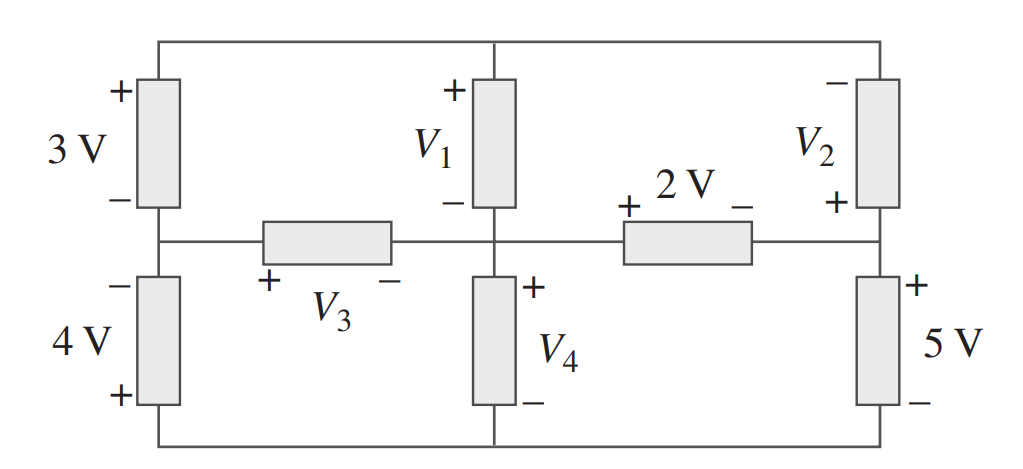
\includegraphics[width=0.8\linewidth]{fig/P2.14.PNG}\cite{charles2013fundamentos}
% \end{frame}

\begin{frame}{Elementos en serie}
    \begin{tabularx}{\linewidth}{X X}
        \begin{itemize}
            \item Dos elementos en serie comparten solamente una de sus terminales y esta no se comparte con un tercer elemento.
            \item Cuando solo existen parejas de elementos en serie en un circuito se le llama circuito en serie.
            \item La corriente en un circuito en serie es la misma para todos los elementos.
        \end{itemize}
        &
        \centering
        \begin{circuitikz} [scale=1]\draw
            (3,0)
                to[R,l=$R_3$,o-]
            (0,0)	
                to[R,l=$R_2$]
            (0,3)
                to[R,l=$R_1$,i^<=$i$,-o]
            (3,3)
            ;
        \draw (1.5,-1.5)node[above, align=left]{$R_{eq}=R_1+R_2+R_3$};
        \end{circuitikz}
    \end{tabularx}
\end{frame}

\begin{frame}{Divisor de voltaje}
    \begin{tabularx}{\linewidth}{X X}
        \begin{gather*}
        v_n = v_T\cdot \frac{R_n}{R_1+R_2+\cdot\cdot\cdot+R_n}\\
        \\
        v_3 = v_T\cdot \frac{R_3}{R_1+R_2+R_3}
        \end{gather*}
        &
        \centering
        \begin{circuitikz} [scale=1]\draw
            (3,0)
                to[R,l=$R_3$,v>=$v_3$,o-]
            (0,0)	
                to[R,l=$R_2$]
            (0,3)
                to[R,l=$R_1$,-o]
            (3,3)
            (3,3)
                to[open,v^=$v_T$]
            (3,0)
            ;
        \end{circuitikz}
    \end{tabularx}
\end{frame}

\begin{frame}{Fuentes de voltaje en serie}
    \begin{tabularx}{\linewidth}{X X}
        \begin{circuitikz} [scale=1]\draw
            (3,0)
                to[V,l=$v_3$,o-]
            (0,0)	
                to[V,l=$v_2$, invert]
            (0,3)
                to[V,l=$v_1$,-o]
            (3,3)
            ;
        \end{circuitikz}
        &
        \centering
        \begin{circuitikz} [scale=1]\draw
            (1,0)
                to[short,o-]
            (0,0)	
                to[V,l=$v_e$]
            (0,3)
                to[short,-o]
            (1,3)
            ;
        \end{circuitikz}
    \end{tabularx}
    \begin{equation*}
    v_{eq} = v_1-v_2+v_3
    \end{equation*}
\end{frame}

\begin{frame}{Elementos en paralelo}
    \begin{tabularx}{\linewidth}{X X}
        \begin{itemize}
            \item Dos o mas elementos en paralelo comparten sus dos terminales.
            \item Cuando solo existen elementos en paralelo en un circuito se le llama circuito en paralelo.
            \item El voltaje en un circuito en paralelo es el mismo para todos los elementos.
        \end{itemize}
        &
        \centering
        \begin{circuitikz} [scale=1]\draw
            (1,3)
                to[short,o-]
            (0,3)	
                to[R,l_=$R_3$]
            (0,0)
                to[short,-o]
            (1,0)
            (0,3) -- (-1.5,3)
                to[R,l_=$R_2$]
            (-1.5,0) -- (0,0)
            (-1.5,3) -- (-3,3)
                to[R,l_=$R_1$]
            (-3,0) -- (-1.5,0)
            (1,3)
                to[open,v^=$v$]
            (1,0)
            ;
            \draw (-1.5,-3)node[above, align=center]{$\frac{1}{R_{eq}}=\frac{1}{R_1}+\frac{1}{R_2}+\frac{1}{R_3}$\\ \\En caso de solo dos resistencias:\\ \\ $R_{eq}=\frac{R_1 \cdot R_2}{R_1+R_2}$ };
        \end{circuitikz}
    \end{tabularx}
\end{frame}

\begin{frame}{Divisor de corriente}
    \begin{tabularx}{\linewidth}{X X}
        \begin{gather*}
        i_n = i_T\cdot \frac{\frac{1}{R_n}}{\frac{1}{R_1}+\frac{1}{R_2}+\cdot\cdot\cdot+\frac{1}{R_n}}\\
        \\
        i_1 = i_T\cdot \frac{\frac{1}{R_1}}{\frac{1}{R_1}+\frac{1}{R_2}+\frac{1}{R_3}}
        \end{gather*}
        En caso de ser solo dos resistencias:
        \begin{equation*}
        i_1 = i_T\cdot \frac{R_2}{R_1+R_2}
        \end{equation*}
        &
        \centering
        \begin{circuitikz} [scale=1]\draw
            (1,3)
                to[short,i=$i_T$,o-]
            (0,3)	
                to[R,l_=$R_3$]
            (0,0)
                to[short,-o]
            (1,0)
            (0,3) -- (-1.5,3)
                to[R,l_=$R_2$]
            (-1.5,0) -- (0,0)
            (-1.5,3) -- (-3,3)
                to[R,l_=$R_1$,i>^=$i_1$]
            (-3,0) -- (-1.5,0)
            ;
        \end{circuitikz}
    \end{tabularx}
\end{frame}

\begin{frame}{Fuentes de corriente en paralelo}
    \begin{tabularx}{\linewidth}{X X}
        \begin{circuitikz} [scale=1]\draw
            (1,3)
                to[short,o-]
            (0,3)	
                to[I,l_=$i_3$]
            (0,0)
                to[short,-o]
            (1,0)
            (0,3) -- (-1.5,3)
                to[I,l_=$i_2$, invert]
            (-1.5,0) -- (0,0)
            (-1.5,3) -- (-3,3)
                to[I,l_=$i_1$]
            (-3,0) -- (-1.5,0)
            ;
        \end{circuitikz}
        &
        \centering
        \begin{circuitikz} [scale=1]\draw
            (1,3)
                to[short,o-]
            (0,3)	
                to[I,l_=$i_e$,invert]
            (0,0)
                to[short,-o]
            (1,0)
            ;
        \end{circuitikz}
    \end{tabularx}
    \begin{equation*}
    i_{eq} = -i_1+i_2-i_3
    \end{equation*}
\end{frame}

% \begin{frame}{Referencias}

% \bibliographystyle{ieeetr}

% \bibliography{referencias}

% \end{frame}

\end{document}
